% !TEX root = thesis.tex

\section{Alguns invariants algebràics}\label{sec:Invariantsalgebraics}

El Teorema \ref{teo:teoremadeReidemeister} dona un mètode per saber quan dos nusos son equivalents, però aquest resultat no permet distingir quan dos nusos son diferents. D'aquesta manera per exemple, encara no sabem que $\ovoid\neq 3_1$. És per això que és necessari la creació d'invariants que ens permetin realitzar aquesta tasca.\\

Recordem que un invariant és un objecte ben definit, ja sigui un número, polinomi, grup, etcètera; que podem associar a un nus qualsevol, de manera que si tenim dos nusos amb diferent valor per aquest invariant, llavors segur que els dos nusos son diferents.

\subsection{L'Ordre}\label{sec:ordrecomainvariant}

Com haviem vist a la Definició \ref{def:ordre}, l'ordre d'un nus és un exemple d'invariant. Nusos amb diferent ordre no poden ser equivalents. Aquest invariant però és quasi intractable a nivell pràctic pel fet d'haver de considerar el mínim nombre de creuaments donats tots els diagrames d'aquest.\\

CAL LA DEMOSTRACIÓ QUE L'ORDRE ÉS UN INVARIANT ALGEBRÀIC (REIDEMEISTER?)

\subsection{El Nombre de Desnuament}\label{sec:desnuamentcomainvariant}

\begin{definition}\label{def:desnuament}
	Diem que $u(K)$ és el \underline{nombre de desnuament} del nus $K$ si aquest és el mínim nombre de canvis en els creuaments d'un nus necessaris per tal d'aconseguir el nus zero donats tots els diagrames de $K$.
\end{definition}

El nombre de desnuament és també un invariant. Aquest però, de la mateixa manera que passa amb l'ordre és intractable a nivell pràctic. Intuïtivament, si $K$ és una corba a $S^3$, llavors $u(K)$ és el mínim nombre de vegades que $K$ ha de passar per sí mateix per aconseguir el nus zero.

\begin{proposition}\label{prop:nombrededesnuament}
	Donat un nus $K$ qualsevol, aquest sempre pot ser desnuat.
\end{proposition}

\begin{proof}
	Entenem per \textit{moviment local} un canvi en els creuaments d'un nus com en el de la Figura \ref{fig:movimentlocal} passant de sobrepassos a sotapassos o a la inversa. D'aquesta manera, recorrent $K$ d'acord amb una orientació qualsevol i fent moviments locals canviant sotapassos a sobrepassos a mesura que aquests van apareixen sense modificar els creuaments que ja haguem visitat ja ho tindriem.
\end{proof}

\begin{figure}
	\centering
	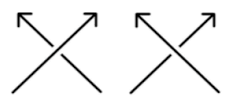
\includegraphics[width=0.6\linewidth]{img/movimentlocal.png}
	\caption{Moviments locals que es poden realitzar en qualsevol creuament d'un nus. A la imatge de l'esquerra, el tros de corda que va de  Sud-Oest fins a Nord-Est passa per sobre de la corda que el creua i doncs en aquest sentit diem que la sobrepassa. A la dreta, aquesta mateixa corda creua per sota i doncs diem que la sotapassa.}\label{fig:movimentlocal}
\end{figure}

\begin{proposition}
	Sigui $K$, $K'$ dos nusos qualssevol, llavors $u(K+K')\leq u(K)+u(K')$
\end{proposition}

\begin{proof}
	És clar que per tal de desnuar $K+K'$ només fa falta desnuar $K$ i $K'$.
\end{proof}

L'altre desigualtat és de fet un problema obert.\\

Per acabar de veure com d'intractable és aquest invariant afirmem el següent resultat sense demostrar-lo.

\begin{proposition}
	Sigui $K$ un nus, existeix un diagrama de $K$ pel qual $u(K)=C$ per a tot $C\in\mathbb{N}$.
\end{proposition}

%CALDRIA DEMOSTRAR QUE SEMPRE EXISTEIX AQUEST NOMBRE (SEMPRE ES POT ARRIBAR AL NUS ZERO CANVIANT UN NOMBRE FINIT DE CREUAMENTS) I QUE AQUEST NOMBRE NO CANVIA SI CONSIDEREM UN ALTRE CREAUMENT (NO IMPORTA EL CREAMENT ESCOLLIT), ENTRE ALTRES RESULTATS.

\subsection{El Gènere}\label{sec:generescomainvariant}

Veurem ara que tot link a $S^3$ es pot veure com la frontera d'una superfície immersa en $S^3$. Aquestes superfícies poden ser utilitzades per estudiar el link.

\begin{definition}\label{def:superficiedeseifert}
	Una \underline{superfície de Seifert} per un link $L$ orientat de $S^3$ és una superfície compacta, connexa i orientable continguda a $S^3$ de manera que la seva frontera és $L$.
\end{definition}

Exemples d'aquestes superfícies son com les de la Figura \ref{fig:superficiedeseifert}. Evidentment, tota superfície compacta connexa i orientada amb frontera dins $S^3$ és un exemple d'un link equipat amb una superfície de Seifert. Una superfície és no orientable si conté una banda de Möbius. Algunes superfícies poden ser construïdes amb un link qualsevol com a frontera de la següent manera: Pintant de color blanc i negre seguint un patró com el d'un taulell d'escacs les regions de $S^2$ que formen el complement del diagrama d'un link. Considerant totes les regions d'un mateix color i juntant-les per bandes amb una mitja volta arribem a obtenir un objecte com el de la Figura \ref{fig:trefoilseifert}.\\

\begin{figure}
	\centering
	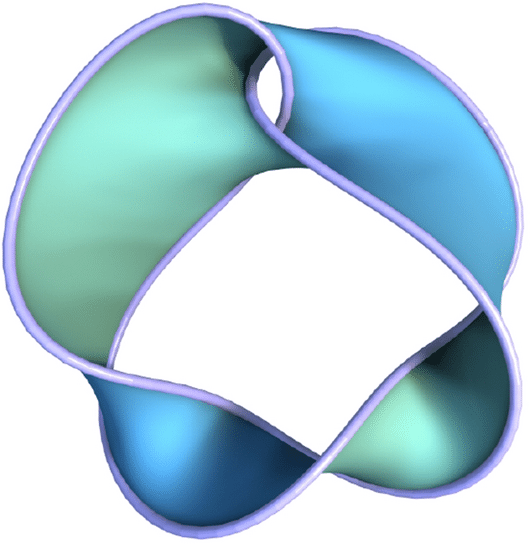
\includegraphics[width=0.6\linewidth]{img/seifertsurface.png}
	\caption{Exemple d'una superfície de Seifert per $5_2$.}\label{fig:superficiedeseifert}
\end{figure}

\begin{figure}
	\centering
	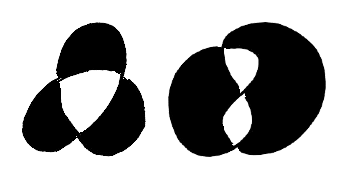
\includegraphics[width=0.6\linewidth]{img/trefoilseifert.png}
	\caption{Dos diagrames del nus $3_1$ pintats com indiquen les instruccions on en comptes de pintar de color negre les regions hem dibuixat línies. Com es pot observar, la superfície de l'esquerra és no orientable mentre que la de la dreta si i doncs és una superfície de Seifert com haviem vist a la Definició \ref{def:superficiedeseifert}.}\label{fig:trefoilseifert}
\end{figure}

Tot i que aquest mètode pot donar resultat a una superfície de Seifert, en general aquest no té perquè ser el cas. Seifert dona un algorisme, per tal de trobar en general una superfície d'aquest tipus.\\

\begin{theorem}\label{theo:existenciadesuperficiesdeseifert}
	Tot link orientat $L$ a $S^3$ té una superfície de Seifert.
\end{theorem}

\begin{proof}
	Sigui $diag(L)$ un diagrama orientat de $L$ qualsevol i sigui $\widehat{diag(L)}$ aquest darrer diagrama modificat segons indica la Figura \ref{fig:movimentsdeseifert}, llavors $\widehat{diag(L)}$ és el mateix que $diag(L)$ excepte en un entorn prou petit de cada creuament on aquest ha sigut eliminat de la única manera possible coherent amb l'orientació. Aquest $\widehat{diag(L)}$ és doncs una unió disjunta de corbes orientades simples i tancades dins $S^2$. Així doncs, $\widehat{diag(L)}$ és la frontera de la unió d'un nombre de discs disjunts tots en un costat de $S^2$. Juntem els discs mitjançant bandes amb una mitja volta als mateixos llocs on hi havia els creuaments. Això forma una superfície orientada amb $L$ com a frontera d'aquesta; cada disc rep la orientació induïda per $\widehat{diag(L)}$ i les bandes que uneixen els diferents discos van alternant aquesta orientació. Si aquesta superfície no és connexa, connectem els components eliminant discos i afegint tubs.
\end{proof}

\begin{figure}
	\centering
	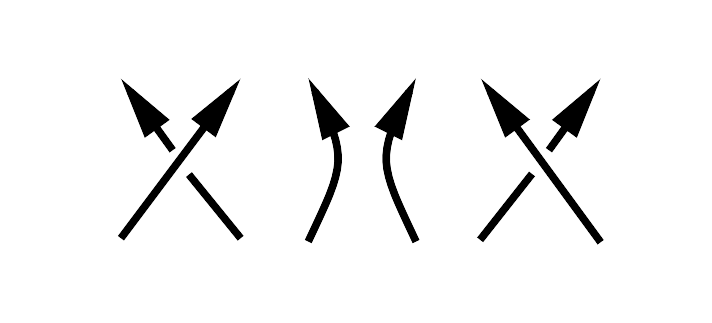
\includegraphics[width=0.6\linewidth]{img/seifert.png}
	\caption{Moviments utilitzats en l'algorisme de Seifert. Quan ens trobem amb un creuament, resoldrem aquest com mostra la imatge central reseguint el nus o link com indica la seva orientació.}\label{fig:movimentsdeseifert}
\end{figure}

En la demostració del Teorema \ref{theo:existenciadesuperficiesdeseifert}, $\widehat{diag(L)}$ era una col·lecció disjunta de corbes simples i tancades construïdes a partir de $diag(L)$. Aquestes corbes s'anomemen \underline{cercles de Seifert} del $diag(L)$. La Figura \ref{fig:cerclesdeseifert} dona un exemple d'aquests.\\

\begin{figure}
	\centering
	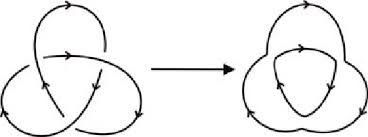
\includegraphics[width=0.6\linewidth]{img/cerclesdeseifert.jpg}
	\caption{Exemple amb la construcció de $\widehat{diag(3_1)}$ a partir d'un diagrama de $3_1$ qualsevol.}\label{fig:cerclesdeseifert}
\end{figure}

Una superfície de Seifert per la Figura \ref{fig:cerclesdeseifert} s'obté afegint dos discos un a sobre l'altre i tres bandes amb una mitja volta cadascun en els creuaments unint així els discos. Evidentment, aquest algorisme dona lloc a una superfície de Seifert donat un diagrama qualsevol de $L$ però aquesta no té perquè ser única. Tampoc té perquè ser la més senzilla donat un diagrama qualsevol.

\begin{figure}
	\centering
	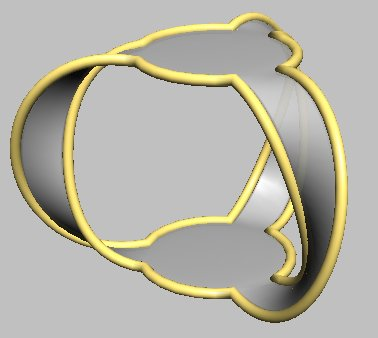
\includegraphics[width=0.6\linewidth]{img/superficiedeseifert.jpg}
	\caption{superfície de Seifert pel nus $3_1$ obtinguda unint els discos amb bandes.}\label{fig:superficiedeseifert2}
\end{figure}

\begin{definition}\label{def:genere}
	El \underline{gènere} $g(K)$ d'un nus $K$ es defineix com $$g(K)=\min\{g(F) \text{: F superfície de Seifert de K}\}$$
\end{definition}

Com en aquest cas $K$ és un nus, $F$ només té un component de frontera de manera que com a superfície abstracte és un disc amb un nombre concret de forats (AIXÒ NO ESTÀ DEL TOT BÉ). A aquest nombre se l'anomena gènere. Més precisament, el gènere de $F$ és $$g(F)=\frac{1}{2}(1-\mathcal{\chi}(F))$$ on $\mathcal{\chi}$ és la característica d'Euler de $F$. La característica d'Euler es pot definir paral·lelament com el nombre vèrtex menys el nombre de costats més el nombre de triangles en qualsevol triangulació de $F$.\\

Si $diag(K)$ té $n$ creuament i $s$ cercles de Seifert, llavors $\mathcal{\chi}(F)=s-n$ de manera que $$g(K)\leq \frac{1}{2}(n-s+1)$$

Aquest invariant té un millor tractament que els vistos anteriorment. A més, no és difícil veure que $K$ és el nus zero si i només si $g(K)=0$. Podem a més trobar una cota superior per aquest gènere. POTSER HAURIEM DE DEMOSTRAR AIXÒ ÚLTIM I A MÉS TAMBÉ DEMOSTRAR QUE EL GÈNERE ÉS UN INVARIANT.\\

\begin{theorem}\label{teo:sumabilitatdelgenere}
	Donats dos nusos $K$ i $K'$, $$g(K+K')=g(K)+g(K')$$
\end{theorem}

\begin{proof}
	JA LA FARÉ
\end{proof}

\begin{corolary}
	Cap nus tret del nus zero té oposat respecte la suma.
\end{corolary}

\begin{proof}
	Suposem que existeix $K$ i $K'$ amb almenys un d'ells diferent del nus zero de manera que $K+K'=\ovoid$, llavors en virtut del Teorema \ref{teo:sumabilitatdelgenere}
	\begin{align*}
		&g(K+K')=g(K)+g(K')\\
		&0=g(K)+g(K')
	\end{align*}
	Com que el gènere d'un nus és un nombre positiu, tenim que $g(K)=g(K')=0$.
\end{proof}

\begin{corolary}
	Hi ha un nombre infinit de nusos diferents.
\end{corolary}

\begin{proof}
	Sigui $K$ un nus no trivial qualsevol i $\sum^{n}K$ la suma de $n$ còpies d'aquest. Veiem que si $n\neq m$, llavors $\sum^{n}K\neq\sum^{m}K$. Suposem que $\sum^{n}K=\sum^{m}K$, aleshores $\sum^{n}g(K)=\sum^{m}g(k)$. Sense pèrdua de generalitat podem suposar que $m>n$, d'aquesta manera $\sum^{m-n}g(K)=0$ cosa que implica $K=\ovoid$.
\end{proof}

\begin{corolary}
	Un nus $K$ amb gènere $1$ és primer.
\end{corolary}

\begin{proof}
	Sigui $K$ un nus amb $g(K)=1$ i expressem aquest com a suma de nusos $K_1$ i $K_2$, llavors $1=g(K_1)+g(K_2)$ i per tant $g(K_1)=0$ o al revés.
\end{proof}

\begin{corolary}
	Tot nus pot ser expressat com a suma finita de nusos primers.
\end{corolary}

\begin{proof}
	Si un nus no és primer, aquest es pot expressar com a suma de dos nusos de menor gènere. Per inducció sobre el gènere ja ho tindriem.
\end{proof}

Es pot veure també, que aquesta expressió és única tret de l'ordenació dels sumands.\\

AL FINAL DE LA SECCIÓ CAL REMARCAR QUE LA TEORIA D'INVARIANTS NO S'HA DE CONCEBRE COM UNA TEORIA ON HI HAGI INVARIANTS MILLORS QUE D'ALTRES, SINÓ QUE CADASCUN AJUDA EN LA CLASSIFICACIÓ DE MANERA QUE EL QUE POTSER UN INVARIANT NO PERMET DISTINGIR, UN ALTRE SI. D'AQUESTA MANERA, PODEM PENSAR EN ELS INVARIANTS COM UNA CAIXA D'EINES QUE PODEM UTILITZAR ALHORA D'ESTUDIAR UN NUS. També m'agradaria tenir una taula amb tots els nusos de fins a 9 creuaments classificats en funció de cada invariant estudiat fins al moment